\begin{surferPage}[Labs]{Een zevendegraadsoppervlak met 99 singulariteiten}
    Oliver Labs construeerde een oppervlak van de graad $7$ toen hij aan zijn thesis aan het werken was, aan Mainz University in 2004. Dit is het huidige wereldrecord voor graad $7$, maar dit zou nog kunnen verbeterd worden: voorlopig weet men enkel dat $\mu(7) \leqslant 104$.
    Labs' oppervlak heeft de symmetrie van een regelmatige zevenhoek (afbeelding links).
    Dit kunnen we goed zien als we van boven naar het oppervlak kijken (afbeelding rechts):

    \vspace*{-0.3em}
    \begin{center}
      \begin{tabular}{c@{\qquad}c}
        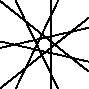
\includegraphics[height=1.5cm]{./../../common/images/labsseptic1.pdf}
        &
        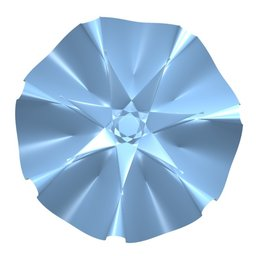
\includegraphics[height=1.5cm]{./../../common/images/labs_septic_von_oben}
      \end{tabular}
    \end{center}
    \vspace*{-0.3em}

    Om dit oppervlak te construeren gebruikte Oliver Labs het computeralgebra-pakket
    {\sc Singular} (Universiteit van Kaiserslautern), dat heel geschikt is voor berekeningen in de algebra\"ische meetkunde en singulariteiten.

    Hij gebruikte hierbij het feit dat we met eindige verzamelingen getallen op een natuurlijke manier kunnen rekenen. Denk bijvoorbeeld aan het lezen van een digitale klok: $24.00$ uur is hetzelfde als $00.00$ uur, en $24.00 + 1.00$ uur is niet $25.00$ uur, maar wel $1.00$ uur. 
\end{surferPage}
